\section{Deployer}
The objective of this section is to give a brief explanation of what is a deployer and how it works. Additionally, some examples of available ones in the market are shown and so is the selected one.
\newline
As introduced above, there must be an adaptor between the rocket and the satellite in order to ensure subjection during the flight, efficient organization of the space in the fairing and a correct separation during the injection maneuver. This duty falls on the deployer. It consists on a prismatic structure prepared to carry the CubeSat inside. When the desired orbit is reached, the deployer uncovers one of its faces so as to let the satellite leave. There is a spring in the bottom that provides a little push to ensure that the CubeSat separates from the rocket. 
There are many types of deployers, some of them are designed for an specific type of mission. As stated before, Electron is compatible with the standard CubeSat deployers, hence, only this type is considered. Similar to the case of the launcher selection, almost all the enterprises don't show enough information on the internet to reach a reliable conclusion, thus, some of them are contacted. Only two answers are obtained, one from ISIS (ISIPOD Deployer) and GAUSS (GPOD deployer). POD stands for Pico-satellite Orbital Deployer. 
\newline
They both present similar characteristics, however there are some differences. First, the main features that both offer are outlined, secondly, the small differences between them are pointed out. 
\begin{itemize}
\item Main features
\begin{itemize}
\item Provide deployment status signal.
\item No battery needed nor external power source
\item No pyrotechnics
\item Protect the CubeSat from external environment
\item Mechanically interfaces with the CubeSats by means of guidelines
\item Mechanically interfaces with the launch vehicle by means of standard fasteners
\item Qualified for multiple of launch vehicles
\end{itemize}
\item ISIPOD 
\begin{itemize}
\item The satellites are fully enclosed inside the deployer, once the CubeSat is fit in, there is no access to it (see image \ref{fig:gull})
\item Electrically interfaces with launch vehicle for telemetry
\end{itemize}
\item GPOD
\begin{itemize}
\item Accessible panels: all the side panels allow the access to the integrated CubSat (see image \ref{fig:tiger}). This means that the entire area between the guide rails over the entire CubeSat length may be freely accessed. 
\item The price for a single deployer 3U is 16000 euros. 
\end{itemize}
\end{itemize}
In order to reach a reliable conclusion, two issues must be taken into consideration. First, the CubeSats of the Astrea Constellation are equipped with thrusters which increase the length of the satellite, thus, the deployer chosen cannot be fully closed. This condition automatically rejects the ISIPOD, nevertheless, there is a second reason for choosing the GPOD, the enterprise ISIS does not show the prices of their deployers even when a request is sent. Without this information it is decided that it cannot be taken into account. 
\newline
\begin{figure}
    \centering
    \begin{subfigure}[b]{0.6\textwidth}
        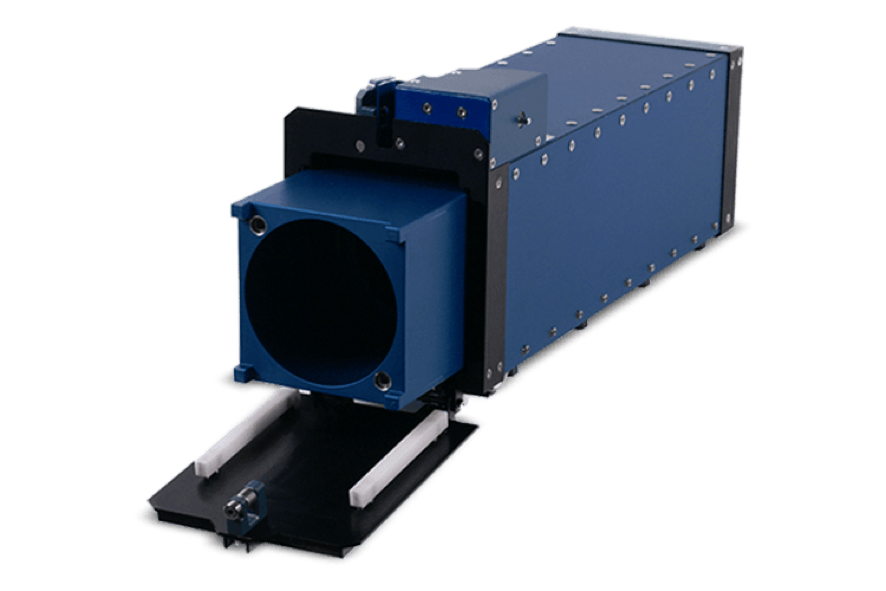
\includegraphics[width=\textwidth]{./Sections_CD/S3-Deployer/Images_S3/Picture_1_S3.png}
        \caption{ISIPOD}
        \label{fig:gull}
    \end{subfigure}
    ~ %add desired spacing between images, e. g. ~, \quad, \qquad, \hfill etc. 
      %(or a blank line to force the subfigure onto a new line)
    \begin{subfigure}[b]{0.6\textwidth}
        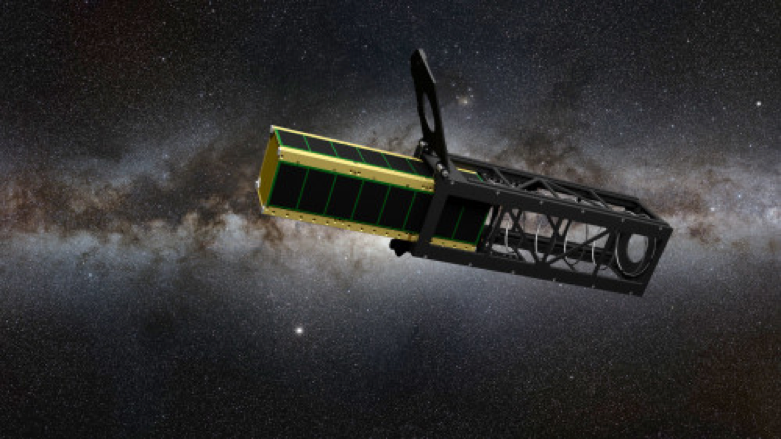
\includegraphics[width=\textwidth]{./Sections_CD/S3-Deployer/Images_S3/Picture_2_S3.png}
        \caption{GPOD}
        \label{fig:tiger}
    \end{subfigure}
    ~ %add desired spacing between images, e. g. ~, \quad, \qquad, \hfill etc. 
    %(or a blank line to force the subfigure onto a new line)
    \caption{Deployer Candidates}\label{fig:animals}
\end{figure}
